% TU Delft Beamer template
% Author: Maarten Abbink
% Delft University of Technology
% March 2014
% Version 2.0
% Based on original version 1.0 of Carl Schneider
\documentclass{beamer}
\usepackage[english]{babel}
\usepackage{calc}
\usepackage[absolute,overlay]{textpos}
% Side by side packages
\usepackage{graphicx,subfig}
% Change margin
\usepackage{changepage}
\mode<presentation>{\usetheme{tud}}

\title{MultiChain}
\subtitle{A cybercurrency for cooperation}
\institute[TU Delft]{Delft University of Technology}
\author{Steffan Norberhuis}
\date{December 14, 2015}

%\setbeameroption{show notes}

\AtBeginSection[] % Do nothing for \section*
{
\begin{frame}<beamer>
\frametitle{Outline}
\tableofcontents[currentsection]
\end{frame}
}


%% Insert frame before each subsection (requires 2 latex runs)
%\AtBeginSubsection[] {
%	\begin{frame}<beamer>\frametitle{\titleSubsec}
%		\tableofcontents[currentsection,currentsubsection]  % Generation of the Table of Contents
%	\end{frame}
%}
%% Define the title of each inserted pre-subsection frame
%\newcommand*\titleSubsec{Next Subsection}
%% Define the title of the "Table of Contents" frame
\newcommand*\titleTOC{Outline}

% define a symbol which can be removed if you don't need it
\newcommand{\field}[1]{\mathbb{#1}}
\newcommand{\Zset}{\field{Z}}

\begin{document}


\setbeamertemplate{navigation symbols}{}

{
% remove the next line if you don't want a background image
\usebackgroundtemplate{
\includegraphics[width=\paperwidth,height=\paperheight]{images/background-titlepage.jpg}}%
\setbeamertemplate{footline}{\usebeamertemplate*{minimal footline}}
\frame{\titlepage}
}\note{
Welcome every one to my defence of my Master's Thesis.
The subject of my thesis is: MultiChain: A cybercurrency for cooperation.
For my thesis I contributed with a first step in a new cybercurrency.
This was done with the Tribler team at the TU Delft.
They develop a peer-to-peer filesharing program.
I will first tell you the outline of my presentation.
}

{\setbeamertemplate{footline}{\usebeamertemplate*{minimal footline}}
\begin{frame}\frametitle{\titleTOC}
	\tableofcontents
\end{frame}
}
\note{
I will start with describing you the problem that the new cybercurrency: MultiChain is trying to solve.
After that I will tell you about the design of MultiChain.
With MultiChain tests were done to validate and evaluate the system.
I will show you the result of these.
As this is a first step, some known vulnerabilities do exist and I will explain these.
I will make some recommendations for future work.
Finally, I will conclude my thesis.
}

\section{Problem Description}

\begin{frame}
\frametitle{Cooperation}
    \begin{definition}
		\emph{Cooperation}* is
		 \begin{itemize}[<+(1)->]
		    \item The action or process of working together to the same end.
		    \item Assitance, especially by complying readily with requests.
		 \end{itemize}
         \uncover<4->{
		    The essence of a collaborative, distributed system is that every node performs tasks for other nodes.
		    }
     \end{definition}
    \begin{figure}
        \centerline{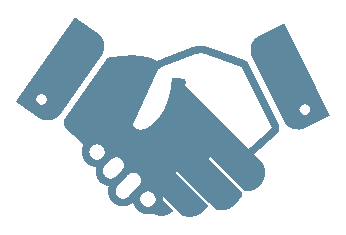
\includegraphics[scale=0.9]{images/problem/handshake.eps}}
    \end{figure}
    * source: The Oxford English Dictionary
\end{frame}
\note{
So lets start with the problem description.
As the subtitle mentioned, MultiChain is to improve cooperation in a peer-to-peer system.
Cooperation is defined as the action or process of working together to the same end.

It is giving assitance upon request.

And this is the essence of a collaborative, distributed system: every participant helps each other.
This system is open to join by any participant.
A peer-to-peer network is such a system.
}


\begin{frame}
\frametitle{Deciding to help}
    \begin{figure}
        \includegraphics<1>[scale=0.3]{images/problem/direct-reciprocity-1.eps}
        \includegraphics<2>[scale=0.3]{images/problem/direct-reciprocity-2.eps}
        \includegraphics<3>[scale=0.3]{images/problem/direct-reciprocity-3.eps}
        \includegraphics<4->[scale=0.3]{images/problem/direct-reciprocity-4.eps}
        \caption{\emph{Direct Reciprocity} between participants.}
    \end{figure}
    \uncover<5->{
        \begin{definition}
            The \emph{Free rider problem} is
            \begin{itemize}
                \item those who benefit from public goods, do not pay for them.
            \end{itemize}
            A private history prevents freeriding in a simple situation.
        \end{definition}
    }
\end{frame}
\note{
But participants do not always help.
Lets take two participants A and B as an example.

A can decide to provide help to B.

And B can return this help.

But he can also choose to not provide this help.

B now benefits from the help of A without contributing back.
The help of A can be seen as a public good.

I now have explained the problem of Free riding to you.
Those who benefit from public goods do not pay for them.

If A remembers that B does not contribute,
he can prevent the freeriding of B by not giving him help in the future.
So a private history can prevent freeriding in the future.

But most often interactions between participants in a peer-to-peer network are one off,
and help cannot be exchanged.
}

\begin{frame}
\frametitle{Help peers that help others}
    \begin{figure}
        \includegraphics<1>[scale=0.3]{images/problem/indirect-reciprocity-1.eps}
        \includegraphics<2>[scale=0.3]{images/problem/indirect-reciprocity-2.eps}
        \includegraphics<3>[scale=0.3]{images/problem/indirect-reciprocity-3.eps}
        \includegraphics<4->[scale=0.3]{images/problem/indirect-reciprocity-4.eps}
	    \caption{\emph{Indirect Reciprocity} between nodes.}
	\end{figure}

	\uncover<5->{
         \begin{definition}
             The \emph{Shadow the Future} prevents A, B, C from deciding not to help.
         \end{definition}
     }
\end{frame}
\note{
Again A can decide to help B,
but he will not want to do so if B never contributes himself.
A will only help peers that help others.
So he will only do that if B himself helps others.

In turn A will only receive help from C if he provided B with help.
This is based upon his reputation for helping B.
A,B,C will be fearful deciding to not help, if they will not receive help themselves in the future.
This is the Shadow of the Future.

But a peer-to-peer system is much larger!
}



\begin{frame}
\frametitle{Public history}
\begin{figure}
	\centerline{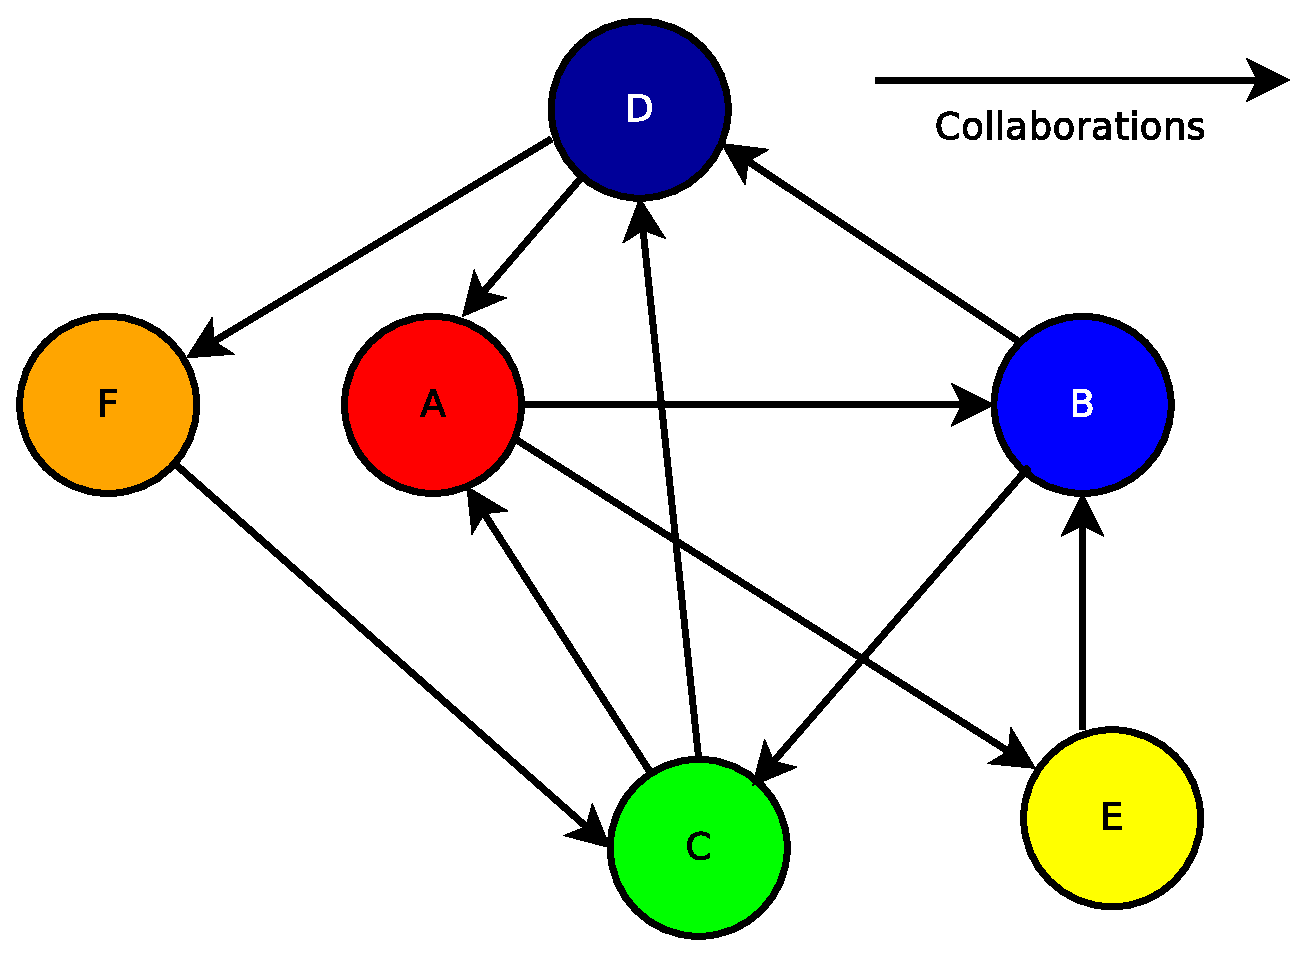
\includegraphics[scale=0.3]{images/problem/network-reciprocity.eps}}
	\caption{\emph{Network Reciprocity} between nodes.}
	\end{figure}
\pause
We need a public, tamper proof interaction history to incentivize collaboration and facilitate trust!
\end{frame}
\note{
You can have a whole network of participants connecting and providing help.
To still prevent freeriding the interaction histories have to be made public.
In such a network a participant can be malicious and we need to prevent his malicious behaviour.

So, we need a public, tamper proof interaction history to incentivize collaboration and facilitate trust!
I now have described you the problem that MultiChain tries to solve.
}

\section{Design}
\begin{frame}
\frametitle{MultiChain}
  \begin{figure}
        \includegraphics<1>[scale=0.3]{images/design/multichain-1.eps}
        \includegraphics<2>[scale=0.3]{images/design/multichain-2.eps}
        \includegraphics<3>[scale=0.3]{images/design/multichain-3.eps}
        \includegraphics<4->[scale=0.3]{images/design/multichain-4.eps}
        \caption{MultiChain blocks chained together and becoming entangled.}
	\end{figure}
	\begin{itemize}
	    \item<2-> The blocks are chained using pointers hash.
	    \item<3-> The chain of A and C are entangled.
    \end{itemize}
\end{frame}
\note{
I will now explain to you the design of MultiChain.

The basis of MultiChain are blocks.
A and B will create a block together.
This contains the data about the interaction between A and B.
I will later describe the contents of the blocks.

This block can be retrieved and inspected by anyone by contacting A or B.
Using this information he will be able to determine the reputation of A and B.

If A and B were to interact again they will create a new block.
This block is chained to the previous block using a hash pointer.
A hash pointer can be described shortly as cryptographic value that describes the block it points to.
Both A and B have an individual pointer that points to the whole, previous block.
This is because A and B both have a chain themselves,
and the previous block could be different blocks.
The design of MultiChain takes a different approach here.
Because we abandon the idea of global ledger, and have indivual ledgers.

A now give help to C,
and A and C now create a block together.
This block will be chained to the previous block of A.
Now the chains of A and C are entangled at the new block.

Also B could interact with another peer D.
}

\begin{frame}
\frametitle{Block creation protocol}
\begin{figure}
	\includegraphics<1>[scale=0.3]{images/design/protocol-1.eps}
	\includegraphics<2>[scale=0.3]{images/design/protocol-2.eps}
	\includegraphics<3>[scale=0.3]{images/design/protocol-3.eps}
	\includegraphics<4>[scale=0.3]{images/design/protocol-4.eps}
	\includegraphics<5>[scale=0.3]{images/design/protocol-5.eps}
	\caption{Sequence diagram for block creation.}
	\end{figure}
\end{frame}
\note{
I will now explain how these blocks are created between A and B.
If A is the uploader he will initiate the block creation protocol with B.
He wants his contribution to be commit to MultiChain.
So he creates a message and adds his data and signature on this message.

He will send this message containing his request.
The request will ask B to add his signature to the block.

B will append his data and his signature. THe block is now created.

B responds with a message containing the block and will immediately add this new block to his chain.

When the message arrives at A he will also add it to his chain.

The block is now present in both chains.
}


\begin{frame}
\frametitle{Contents of a block}
\begin{figure}
    \begin{adjustwidth}{-1em}{0em}
    \includegraphics<1>[scale=0.25]{images/design/signatures-1.eps}
    \includegraphics<2>[scale=0.25]{images/design/signatures-2.eps}
    \includegraphics<3>[scale=0.25]{images/design/signatures-3.eps}
    \includegraphics<4>[scale=0.25]{images/design/signatures-4.eps}
    \includegraphics<5>[scale=0.25]{images/design/signatures-5.eps}
    \includegraphics<6>[scale=0.25]{images/design/signatures-6.eps}
    \includegraphics<7>[scale=0.25]{images/design/signatures-7.eps}
    \includegraphics<8->[scale=0.25]{images/design/signatures-8.eps}
    \end{adjustwidth}
	\caption{All 14 fields in a MultiChain block.}
	\end{figure}
	\uncover<9->{
	    \begin{itemize}
	        \item Signatures have the property of non-repudiation. Authors cannot revoke their authorship.
	    \end{itemize}
	}
\end{frame}
\note{
I will now describe to you the contents of a block.
First part is the up field.
This field contains the amount of data uploaded in MegaBytes by the uploader A.

The second part is the down field.
This contains the amount of data transferred back to A.

The public keys of A and B indentify A and B and are added to the block.

The total up and total down of A for the whole chain is added.

The hash pointer of A  and a sequence number that identifies the block number in the chain of A.

This is all the data supplied by A.

Next, the total up and total down of B is added by B.

Also the hash pointer and sequence number of B is added.

The block contains the signature of A and B.
The signature of A is only on part of the block.
While B signs the whole block.

Because A and B signs the block they announce that it is truthfull and cannot later renounce that statement.
This is called non-repudiation.
}

\begin{frame}
\frametitle{Size of a block}
    \begin{figure}
        \begin{adjustwidth}{-1em}{0em}
            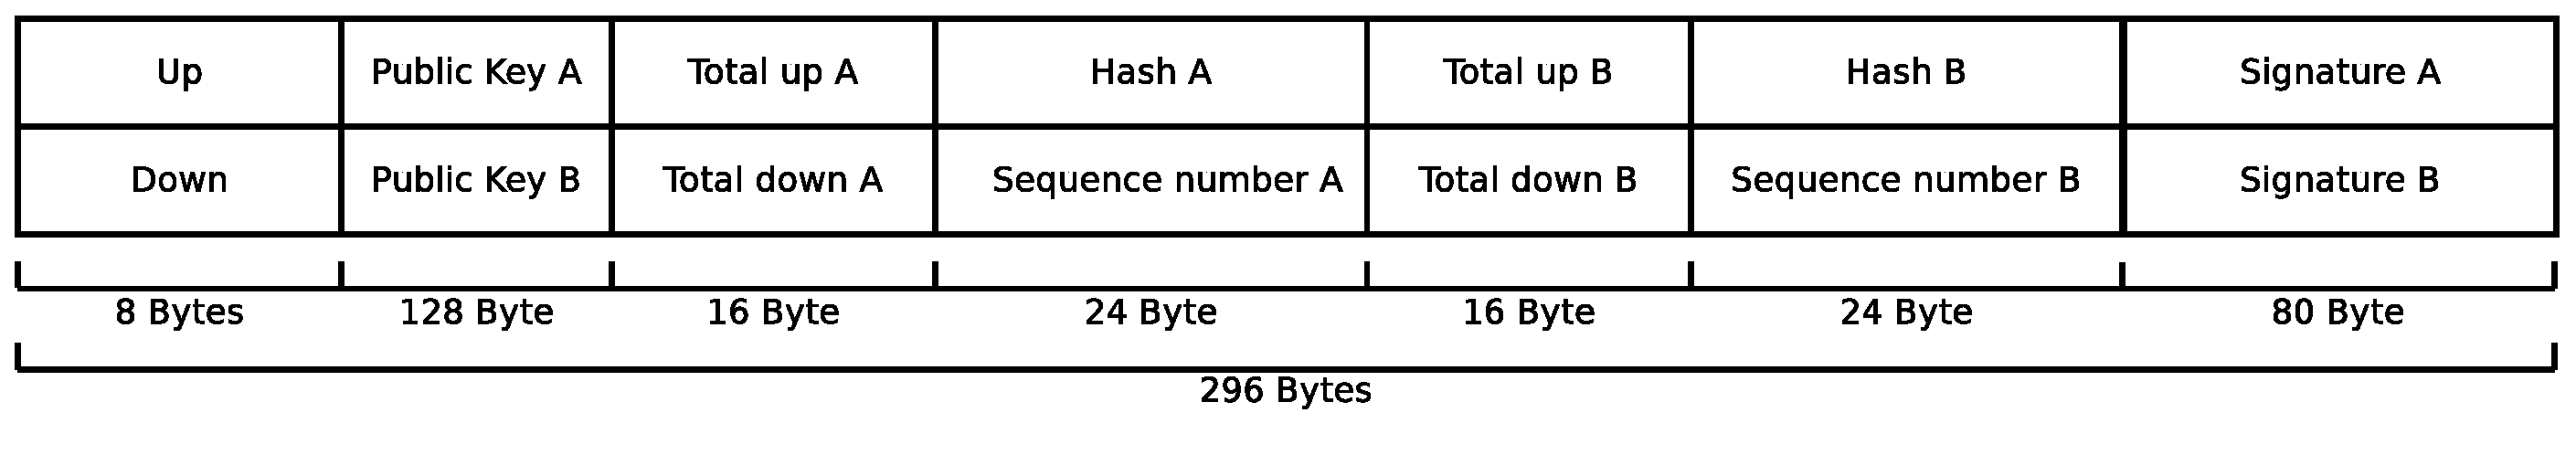
\includegraphics[scale=0.25]{images/design/size.eps}
        \end{adjustwidth}
            \caption{Size of a block in MultiChain.}
        \end{figure}
    \begin{itemize}
        \item The size of a block is important as it will determine how fast the data structure grows.
        \pause \item The size is dependent on the hashing algorithm and signature algorithms.
    \end{itemize}
\end{frame}
\note{
The size of the blocks are important.
If they are too big, the datastructure will grow too fast.
MultiChain will not be usable on small devices and will not be scalable.

Here an overview of the subcomponent size is shown.
Most of the size is due to the cryptographic components added to the block.
This is determined by the hashing algorithm and signature algorithms used.

The size of the counters determine how much data MultiChain can track.
The upper limit in total is 4.6 x10^9 petabytes.
So this is sufficient for the future.
}

\begin{frame}
\frametitle{Atomic operations on the chain}
    \begin{itemize}
        \item A chain is immutable and can only be appended to.
        \pause \item Only atomic operations are allowed on the chain. This prevents branches.
        \pause \item A peer drops any incoming requests during outstanding request. This is a Drop Event.
    \end{itemize}
\end{frame}
\note{
The chain is immutable and can only be appended to.

Only atomic operations are allowed on the chain. This prevents branches.

A peer drops any incoming requests during outstanding request. This is a Drop Event.
He cannot process that request, because only atomic operations are allowed.
}

\begin{frame}
\frametitle{Half signed blocks}
    \begin{figure}
        \includegraphics<1>[scale=0.3]{images/design/halfsigned-chain-1.eps}
        \includegraphics<2>[scale=0.3]{images/design/halfsigned-chain-2.eps}
        \includegraphics<3>[scale=0.3]{images/design/halfsigned-chain-3.eps}
        \includegraphics<4>[scale=0.3]{images/design/halfsigned-chain-4.eps}
        \includegraphics<5->[scale=0.3]{images/design/halfsigned-chain-5.eps}
        \caption{A chain of with a half signed block in MultiChain.}
	\end{figure}

\end{frame}
\note{
But there is a problem in the protocol that arises from the fact that it is used in a asynchronous system.
There is no way of synchronizing with absolute certainty that both A and B commit their block to the chain.
A gives out a message to B to create a block.
B create this block at any moment he desires.

This causes the problem that A would have to wait indefinetly until B responds to create a new block.
As only atomic operations are allowed.
If A would continue, then A would create a branch in his chain if B does create a block.
But B could fail or be malicious and deny A his response.

A major contribution of my thesis is the solution to this problem.
We introduce the notion of a half signed block.

So A and B have created a block like before.
A will wait on B until a certain period expires.
If B does not respond within this period, A will create a halfsigned block.
The part of B is missing.
After that A can continue interacting with for example C.

It is possible that B did create the block, but was to late to respond fast enough.
This block is still added to the chain of B.
There is now an inconsitency between A and B.
But A gives proof that he tried to create a block and is not double spending.
The block is initiated by A and is therefore beneficial for him to exist.
So this beneficial inconsitency is acceptable in a reputation system.

B chains does continue using the full block.
A does not include the full block.
}

\section{System tests and evaluation}

\begin{frame}
\frametitle{Evaluating downloads at different speeds}

\begin{figure}
\centerline{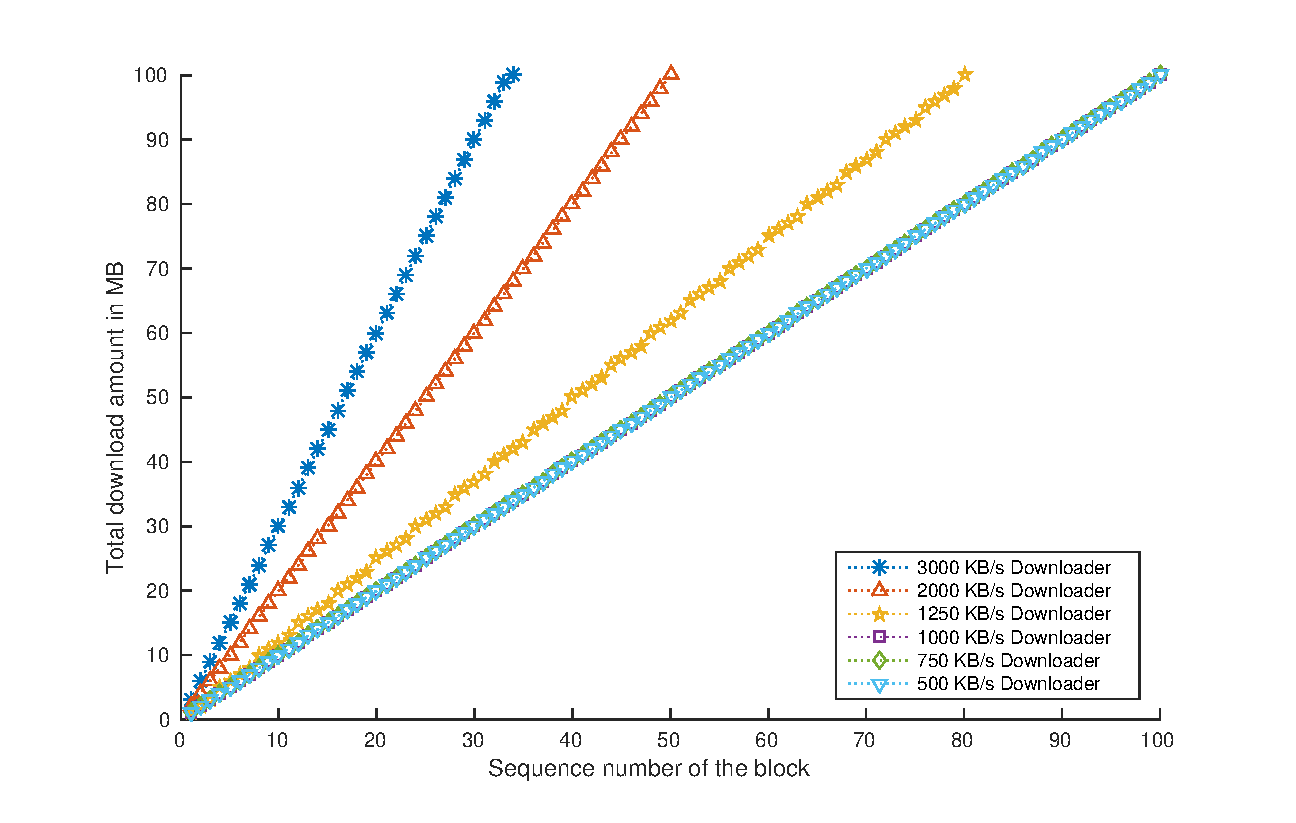
\includegraphics[scale=0.5]{images/experimentation/synthetic-simple-down.eps}}
\caption{Total download amounts repeated 6 times with different speeds.}
\end{figure}
\end{frame}
\note{
The first experiment that I will describe is a simulation of a download between a uploader and a downloader.
A file of 100 MB is repeatedly downloaded at different speeds.
The download transcribed in the blocks are plotted.
Important to note is that the x axis does not plot time,
but the number of blocks used.
Upload amounts are only updated every second because of limitations of the simulation.

But MultiChain will wait for a certain amount of data before it would schedule a block anyway.
Because MultiChain is designed to only schedule to create blocks above a certain threshold.
That is why there are three overlapping lines at 1 MB every block.
This is exactly the threshold.
We call this The Scheduler Effect.

The speed increase above the threshold can be seen in the slope of the figures.
Also the numbers of blocks needed for the download is less.

There are no discontinuities in the graph.
MultiChain has no problem in keeping up with the traffic
and correctly transcribes the traffic.
}

\begin{frame}
\frametitle{Anonymous downloading}

\begin{figure}
	\centerline{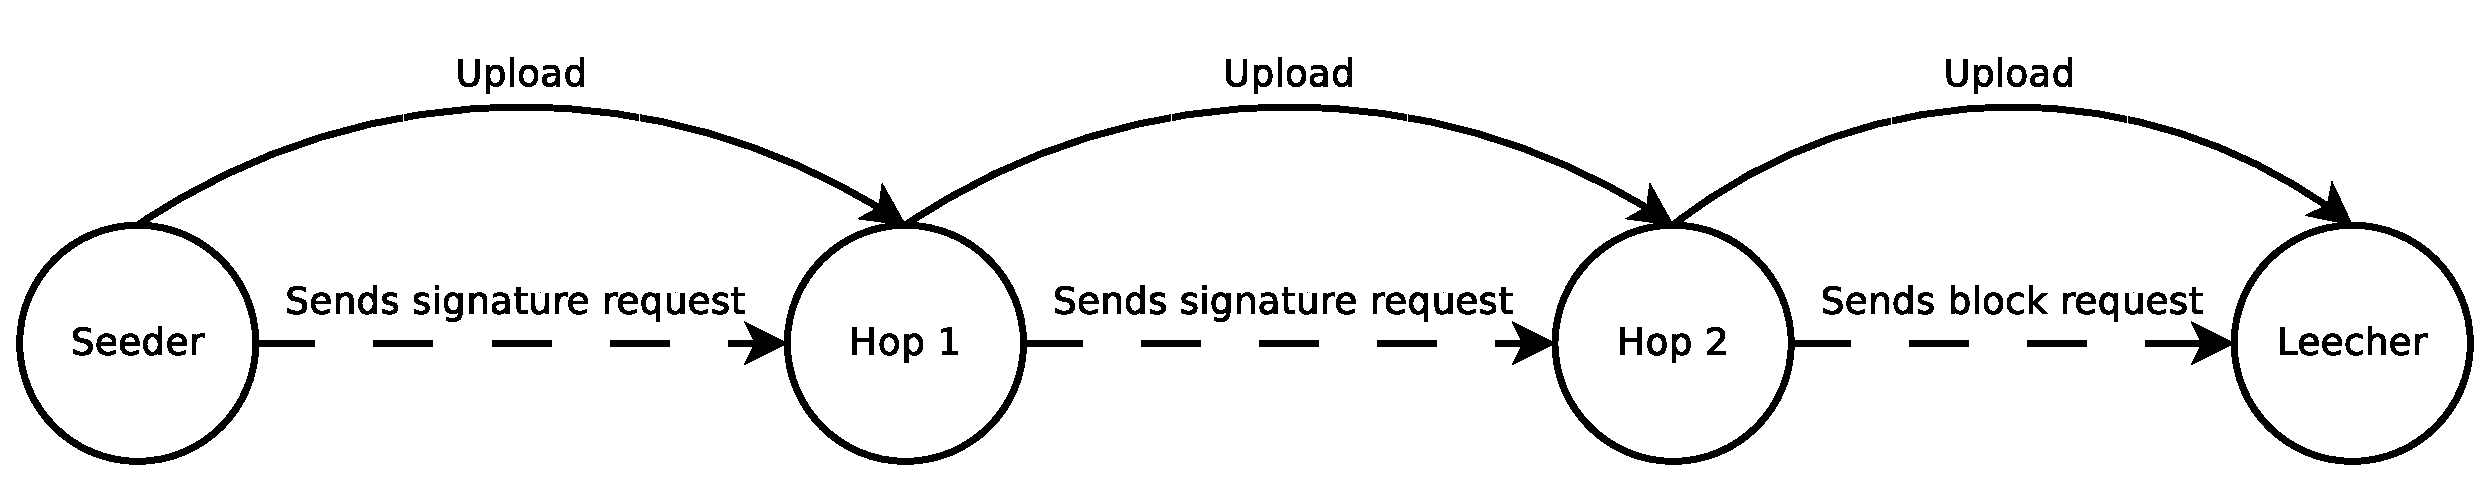
\includegraphics[scale=0.25]{images/experimentation/seeder-hops-downloader.eps}}
	\caption{Block creation in an anonymous download.}
	\end{figure}
\end{frame}
\note{
MultiChain was developed to be used to track anonymous downloading.
This is a more complicated situation that I will explain.
In anonymous downloading the data is transferred through intermediate hops.
These hops relay the data to a next hop.
The number of hops can be varied to increase anonymity at the cost of download speed.

We also simulated this situation to evaluate MultiChain.
}

\begin{frame}
\frametitle{Anonymous download experiment}

\begin{figure}
    \centering
    \begin{adjustwidth}{-3em}{-3em}
    \subfloat[]{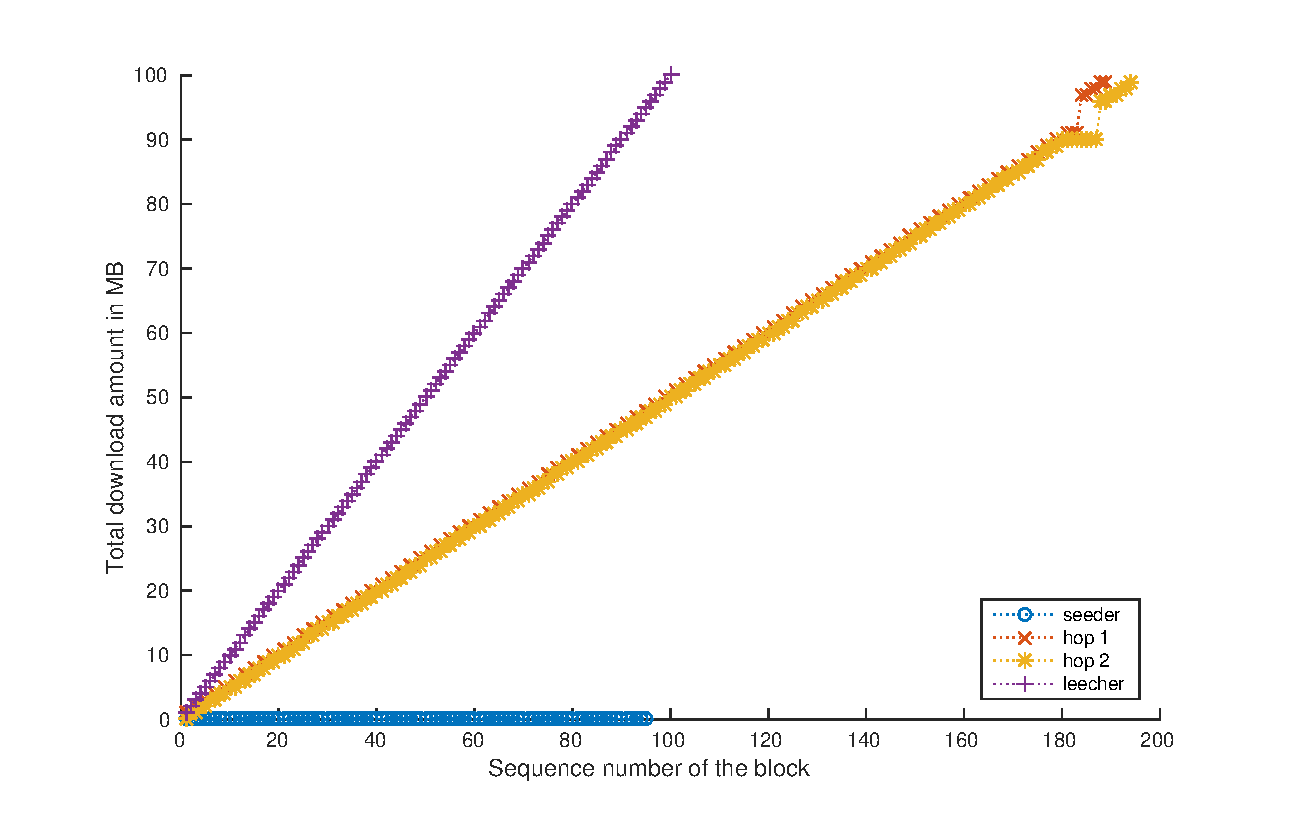
\includegraphics[trim={.5cm 0cm 0cm 0cm},clip=true,width=.46\linewidth]{images/experimentation/synthetic-anonymous-down.eps}}\hspace{0em}%
    \subfloat[]{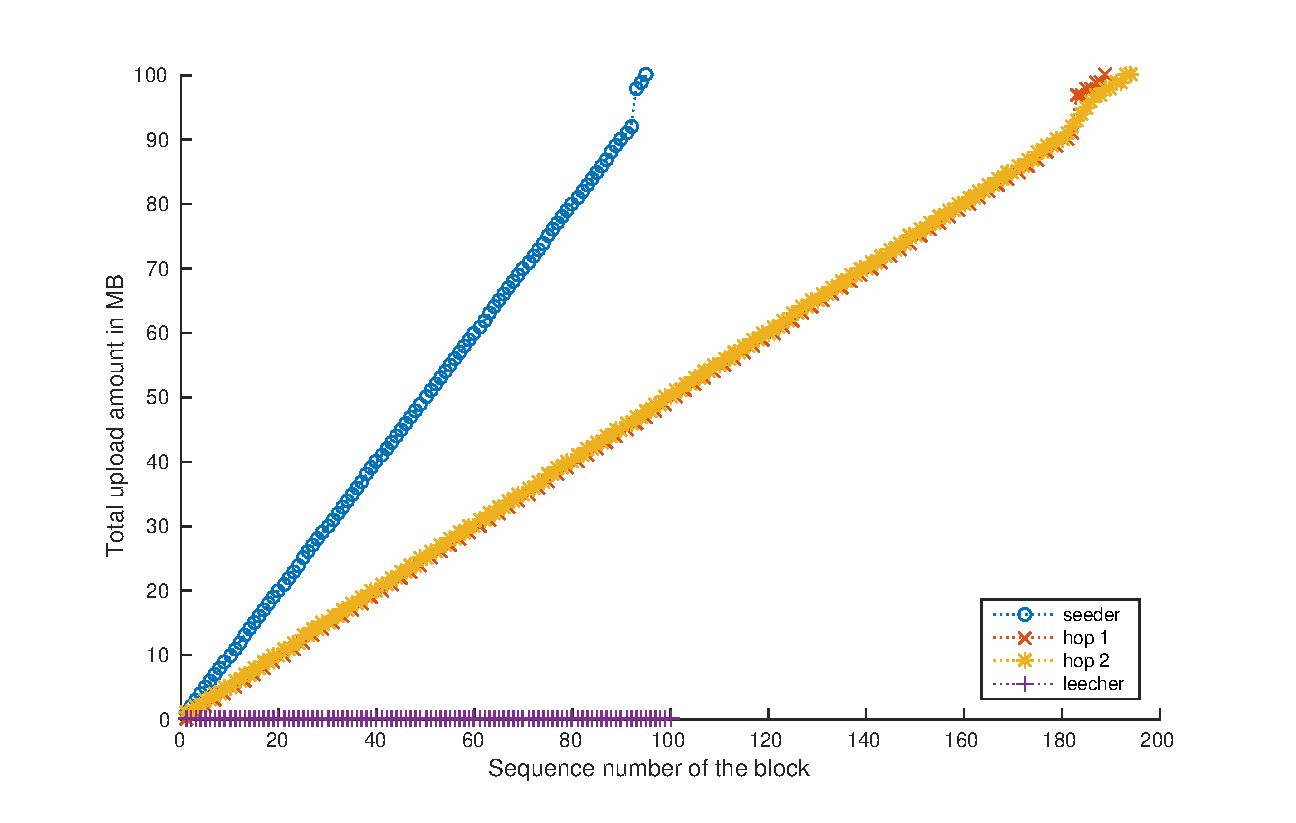
\includegraphics[trim={.5cm 0cm 1cm 0cm},clip=true,width=.46\linewidth]{images/experimentation/synthetic-anonymous-up.eps}}
    \end{adjustwidth}
    \caption{Download and upload amounts during the anonymous download experiment.}
\end{figure}
\end{frame}
\note{
Here the result of the experiment are plotted.
Again the download of every block is plotted on the left, Now the upload amounts are also plotted on the right.
MultiChain correctly tracks the download without problems until 92% of the download.

Here we a drop event occurs.
A request by hop 1 is dropped by hop 2.
Hop 1 has to wait for the timeout and in turns causes the uploader to experience a dropevent.
Meanwhile hop 2 and the downloader continue to track their download amounts.
This can be seen in the plot.
The download as a whole is not paused due to the dropevent.
Only the tracking of amounts is postponed.

Later you see MultiChain to correctly recover and continue tracking amounts.
MultiChain is able to track anonymous downloads.
}


\begin{frame}
\frametitle{Entanglement in an anonymous download}
\begin{figure}
    \centering
        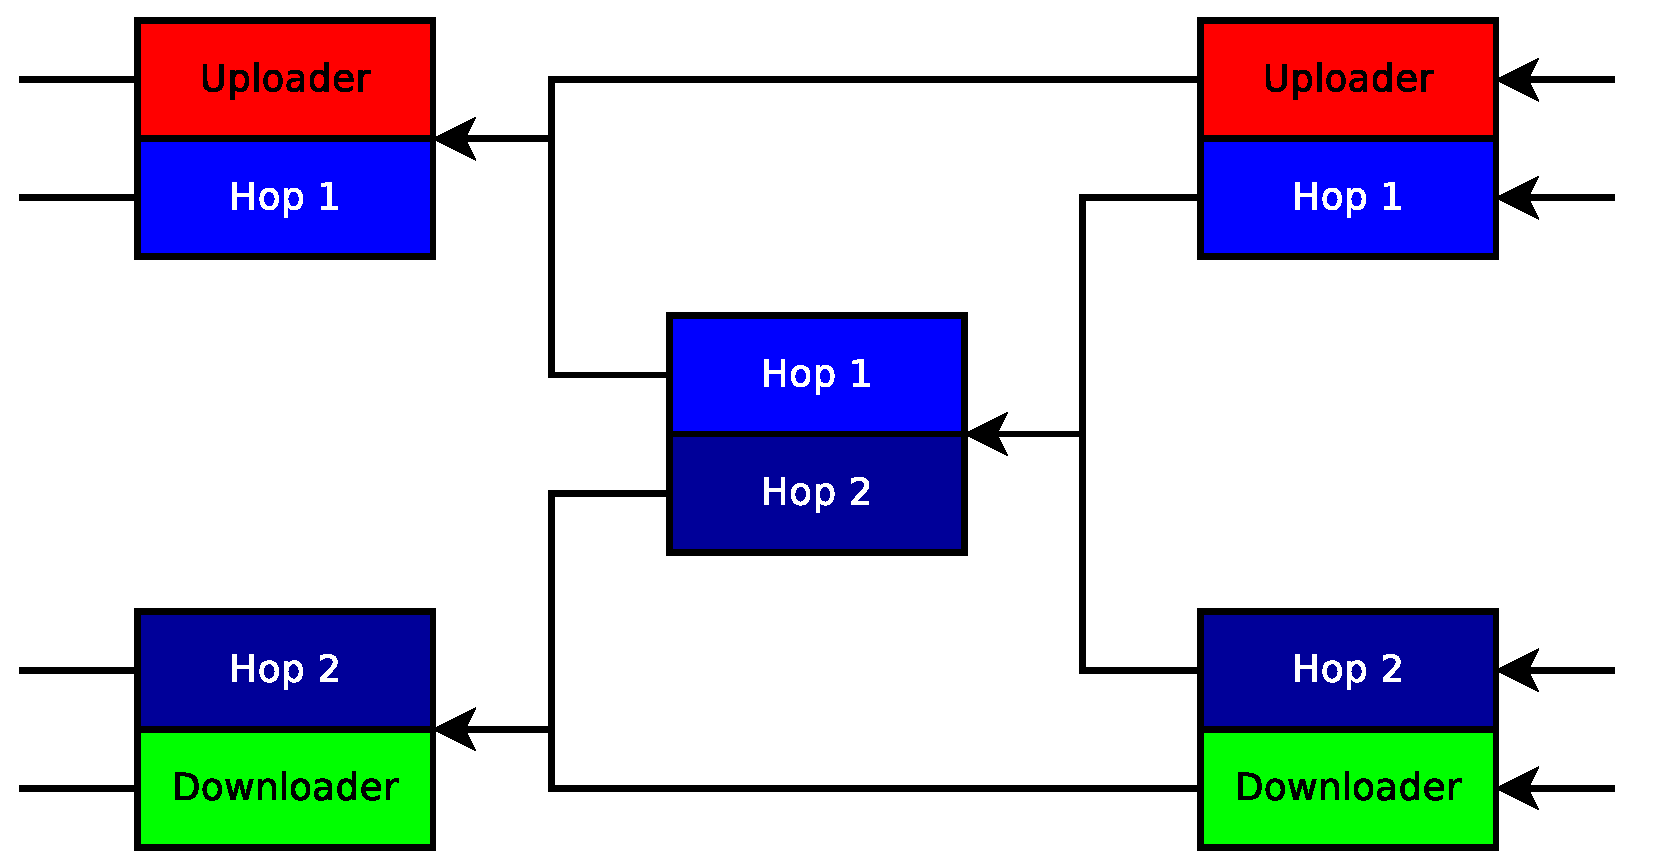
\includegraphics[scale=0.3]{images/experimentation/anonymous-chain.eps}
    \caption{Entanglement}
\end{figure}
\end{frame}
\note{
Here a diagram is shown about how the MultiChain will be constructed during the experiment.
The uploader creates blocks with the first hop.
The first hop creates in turn blocks with the second hop.
This second hop creates blocks with the downloader.
This results in the following structure that shows the entanglement of chains.
}

\begin{frame}
\frametitle{Dropevent in an anonymous download}
\begin{figure}
    \centering
        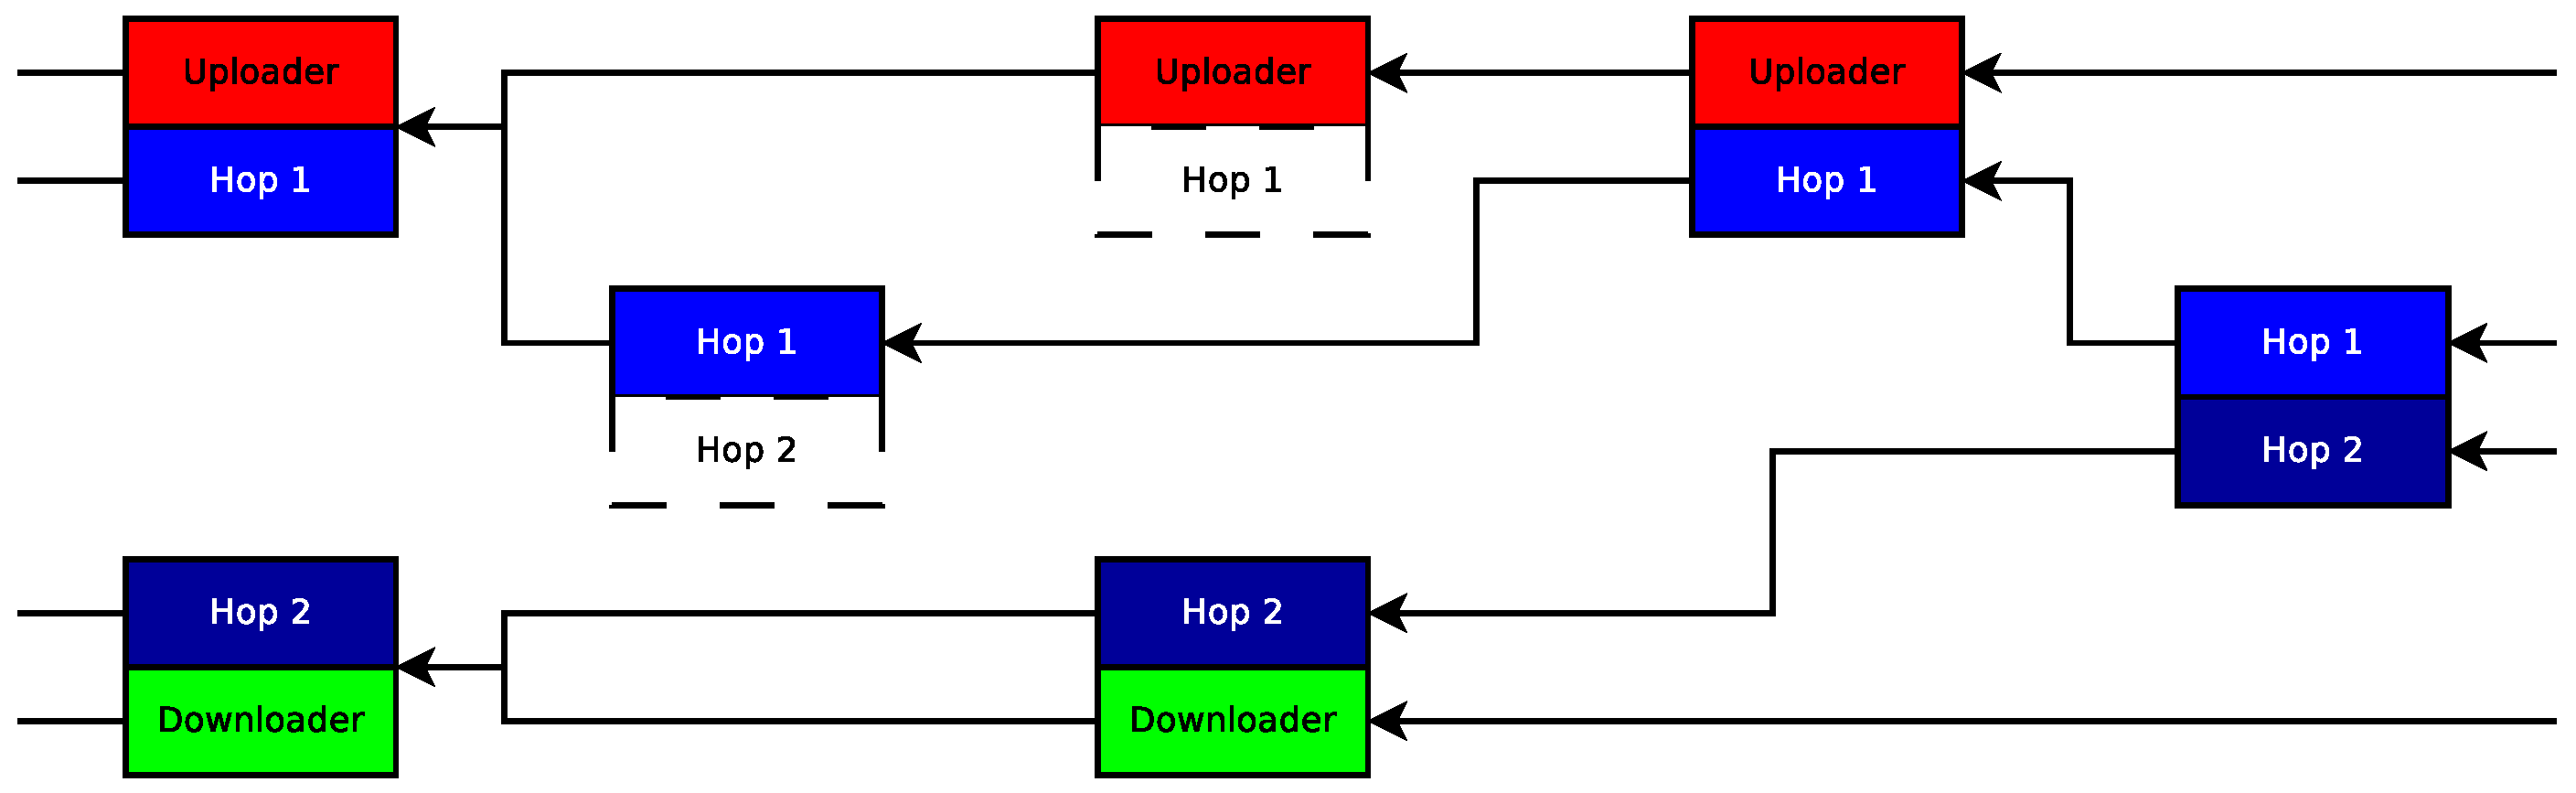
\includegraphics[scale=0.2]{images/experimentation/anonymous-dropevent.eps}
    \caption{Drop event structure}
\end{figure}
\end{frame}
\note{
During the drop event,
the structure changes.
Half signed blocks are created while hop 2 and the downloader continue creating blocks.
When MultiChain recovers the normal structure continues.
}


\section{Known vulnerabilities}

\begin{frame}
\frametitle{Double spending}
\begin{figure}
	\includegraphics<1>[scale=0.3]{images/vulnerabilities/branch-multiple-1.eps}
	\includegraphics<2>[scale=0.3]{images/vulnerabilities/branch-multiple-2.eps}
	\includegraphics<3->[scale=0.3]{images/vulnerabilities/branch-multiple-3.eps}
	\caption{Double spending by M.}
\end{figure}
\end{frame}
\note{
I will now discuss with you the known vulnerabilities of MultiChain
The malicious node can have a block with A he is unhappy with.
This could be because that block records a huge download of him.

He will forget this chain and create a new branch.
His freeriding will not be exposed and he can continue his abuse.

He can even do this multiple times.
But if some one has both blocks containing the same hash pointer,
his fraud will be exposed.
}

\begin{frame}
\frametitle{Sybil attack}
\begin{figure}
    \includegraphics<1>[scale=0.3]{images/vulnerabilities/sybil-1.eps}
	\includegraphics<2->[scale=0.3]{images/vulnerabilities/sybil-2.eps}
	\caption{The sybil attack by M.}
	\end{figure}
\end{frame}
\note{
Another known vulnerability is The Sybil Attack.
This is a well known attack within reputations systems that has not yet been solved.
For example this could be an example of the chain of the malicious node.
This chain shows him contributing to A, B, C, and D.

But in reality: A,B,C,and D are just fake identities created by the malicious node that report fake contributions.
}
\section{Recommendations}
\begin{frame}
    \frametitle{Recommendations}
    \begin{itemize}
        \item Add queuing to minimize drop events.
        \pause \item Create fungible reputations to increase anonymity.
        \pause \item Crawl the network looking for double spending proofs and broadcast these proofs in the network.
        \pause \item Look for outgoing edges of Sybil networks.
    \end{itemize}
\end{frame}
\note{
So now I will shortly summarize some recommendations I have for the next steps to improve  MultiChain.

First, a queue should be added that prevents messages to be dropped. This reduce the occurances of drop events.

Secondly, reputations should be made transferable in a special block.
This will create fungible reputations and increase anonymity.

The network can be crawled looking for double spending proofs.
These proofs can be used to punish peers by excluding them from the network.

Sybil attacks will create a network of identities all refering to themselves.
Outgoing edges will most likely be easy to spot and can be used to identify Sybil Attacks.
}

\section{Conclusion}

\begin{frame}
\frametitle{Conclusion}
\begin{itemize}
    \item{Difficult to make a scalable reputation system. But a different approach of individual ledgers can work.}
    \pause \item{Experiments shows that MultiChain has promise to be a scalable reputation system.}
    \pause \item{A lot of work is still needed to provide adequate security within MultiChain.}
\end{itemize}
\end{frame}


\end{document}
